\chapter{Implémentation}
\label{chap:implem}
Dans ce chapitre nous aborderons les problématiques lié à l'implémentation. Nous allons, dans un premier temps, évaluer les contraintes liés au support d'implémentation et dans un second temps les conversions que nous avons effectuer pour que l'entrée et la sortie de notre commande correspondent puissent être utilisé sur le micro-contrôleur. Finalement, nous expliquerons notre implémentation.\\

Voici, ci-dessous figure \ref{fig:GeneralSCHEMA}, le schéma général des différents éléments.	
\begin{figure}[!ht]
\centering 
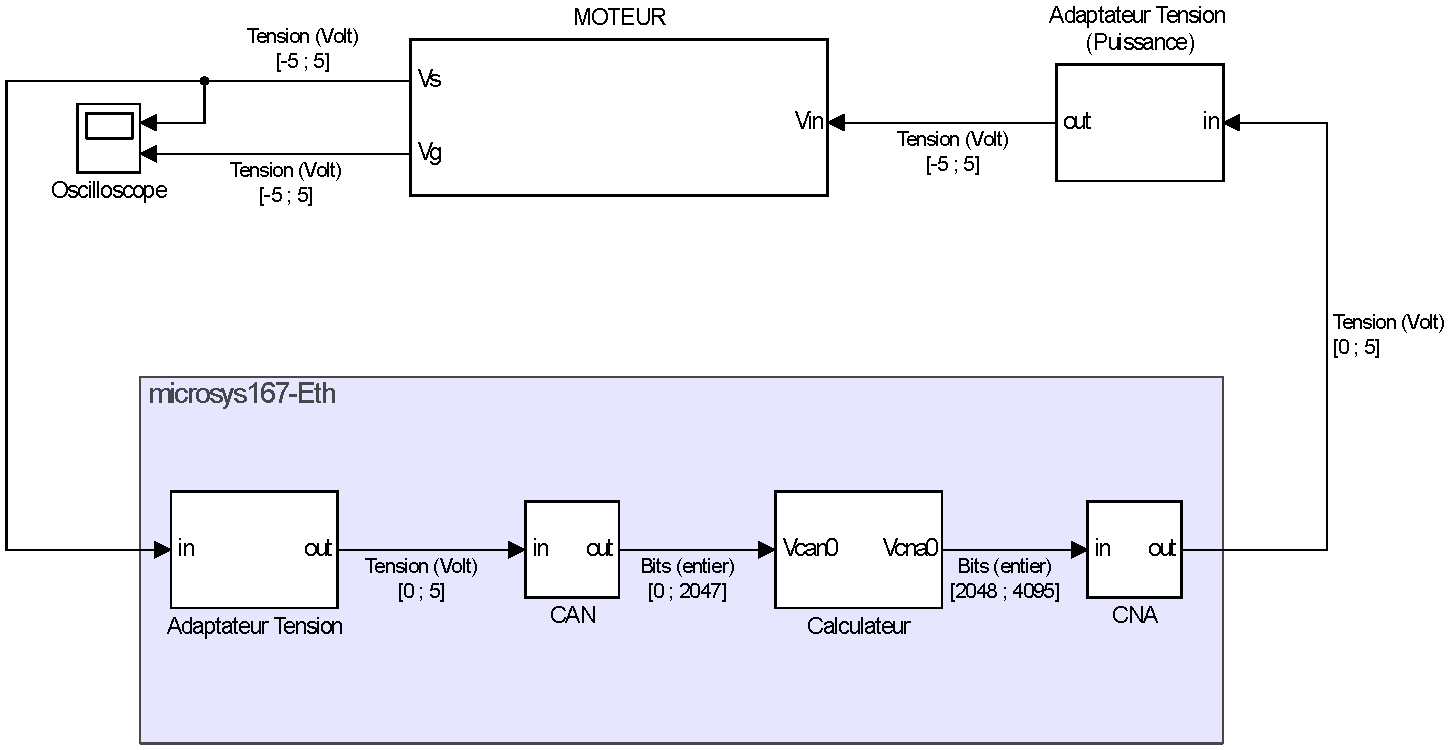
\includegraphics[width=.7\textwidth]{./V/images/schemaMO_MICRO.pdf}
\caption{\label{fig:GeneralSCHEMA}Schéma des différents composants du montage.}
\end{figure}
On remarque qu'il y a 4 composants et le détail, non exhaustif, des éléments utiles de la carte \emph{microsys167-Eth}.
Le bloc nommé moteur correspond au banc moteur présent en salle de TP. Le scope correspond à l'oscilloscope. Le bloc adaptateur de tension (Puissance) est la carte qui permet de passer de la tension de commande ($0$ à $5$ Volt) vers une tension adaptée au moteur ($-5$ à $5$ Volt).
\section{Contraintes hardware} 
Nous allons, dans cette partie, nous consacrer à une étude des contraintes matérielles. Dans un premier temps nous verrons quels sont les spécificités du micro-contrôleur. Puis, nous verrons les convertisseurs analogique/numérique et numérique/analogique et nous conclurons sur le choix du micro-contrôleur. 
	\subsection{Micro-contrôleur C167}
		%(ordo,taches,validation TR,temps calcul, fréquence fonctionnement)
Pour ce projet, nous disposons d'un micro-contrôleur \emph{C167} fabriqué par Siemens. Il est dans une carte \emph{microsys167-Eth} qui lui  ajoute des interfaces, des fonctionnalités et de la mémoire. La carte cadence le micro-contrôleur à $20\text{ }MHz$, ajoute un $1\text{ }Mo$ de RAM et $512\text{ } Ko$ de Flash-EPROM. Nous disposons aussi d'adaptateurs de tension ($\left[-5;5\right]$ Volt vers $\left[0;5\right]$ Volt). Le \emph{C167} offre différentes fonctionnalités, dont les interruptions matérielles, les taches, les timers périodiques et un débogueur. Nous avons également des outils de développement permettant depuis un ordinateur, de créer un programme en \emph{C}, le compiler pour le \emph{C167}, l'envoyer sur celui-ci et si besoin de le déboguer et récupérer des valeurs sur un terminal. La fréquence de fonctionnement du \emph{C167} est de $20 $ MHz et un cycle instruction faut 4 cycle CPU, donc la fréquence d'instruction est de $5 $ MHz.
Le \emph{C167} a également des entrées et des sorties numériques et analogiques. Nous allons maintenant vous parlez des problématiques de conversions.
	\subsection{CAN / CNA\label{sub:CAN_CNA}}
%		(protocole correction, temps conversion, échantillonnage bits )	
\subsubsection{CAN}
%%%% CAN			
Nous allons détailler deux types de conversions nécessaires à ce projet. \\
\hspace{3mm} \textbf{CAN :} (Conversion Analogique Numérique.) Durant cette opération, le convertisseur échantillonne grâce à un bloqueur (discrétisation temporelle) puis quantifie (discrétisation de l'amplitude) le signal analogique. Il restitue un signal numérique après un temps de conversion $t_{CAN}$. Nous avons besoin de ce type de convertisseur pour la lecture des entrées dans notre cas, $V_{D}$. La qualité de notre conversion dépend de plusieurs éléments : 
\begin{itemize}
\item Le nombre de bits de sortie (la sortie ne pouvant prendre que $2^{\text{nbrBit}}$ valeurs différentes). Nous avons des CAN 11 bits.
\item La fréquence de conversion du signal analogique $f_{e}$ par rapport à la fréquence utile maximale du signal a convertir $f_{max}$. Le théorème de Shannon préconise d'avoir au moins le rapport de l'équation \ref{equ:Fshannon}, en pratique nous respecterons le rapport de l'équation \ref{equ:Freel}. Cela évite le repliement.
\begin{eqnarray}
\label{equ:Fshannon} f_e &>& 2*f_{max}\\
\label{equ:Freel} f_e & \approx & 5*f_{max}
\end{eqnarray}
Nous avons considéré que la fréquence utile maximale de la position d'un moteur à courant continue est d'environ $f_{max} = 100Hz$. Nous avons donc pris :
\begin{eqnarray}
\label{equ:fe}f_e &=& 520\text{Hz}\\
\label{equ:Te} T_e &=& 52 \text{ms}\\
\end{eqnarray}
\item La conversion doit être linéaire. En effet, il existe différentes erreurs possibles. Il peut y avoir un offset, une erreur de gainn une non-linéarité intégrale ou différentielle (voir figure \ref{fig:errCAN}).
\end{itemize}
\begin{figure}[!ht]
\centering 
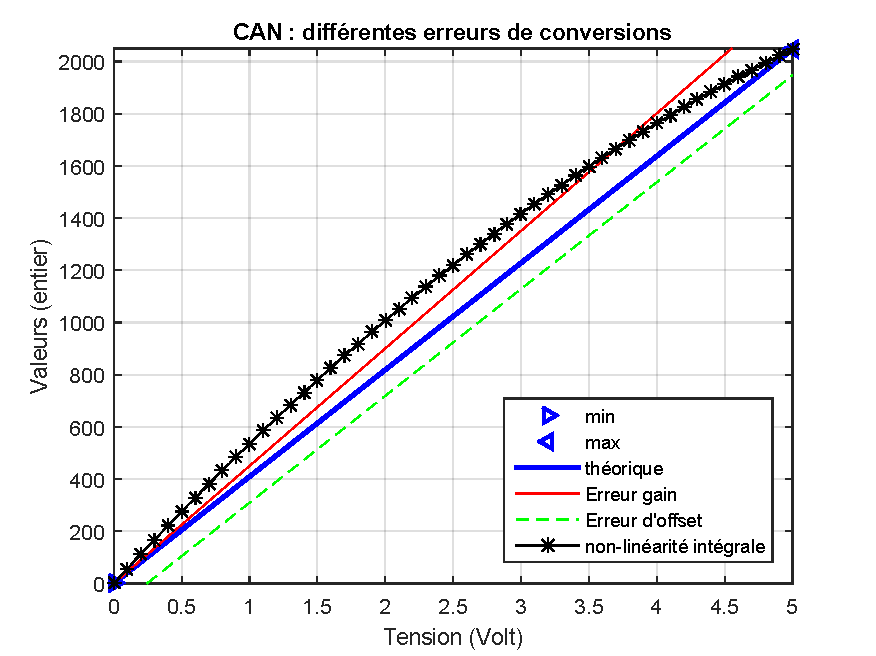
\includegraphics[width=.6\textwidth]{./V/images/CAN.pdf}
\caption{\label{fig:errCAN}Erreurs de conversions possibles sur le CAN}
\end{figure}
\subsubsection{CNA}
\hspace{3mm} \textbf{CNA :} (Conversion Numérique Analogique.) Ici, le convertisseur transforme le signal numérique en un signal analogique après un temps de conversion $t_{CNA}$ (équation \ref{equ:tcan}). Nous avons besoin de ce type de convertisseur pour la génération de la sortie dans notre cas, $V_{s}$. La qualité de notre conversion dépend de plusieurs éléments similaires au CAN. L'entrée du CNA est un entier codé sur 12 bits et il génère une tension comprise entre $-5$ et $5$ Volts. 
\begin{eqnarray}
\label{equ:tcan}
t_{CAN} &=& 14*t_{cc} + 2*t_{sc} + 4*TLC \\
&=&  9,7 \mu s%\\
%T_{CNA} &=& %% TODO %%%%%%%%%%%%%%%%%%%%%%%%%%%%%%%%%%%%%%%%%%%%% /!\  %%%%%%%%%%%%%%%%%%%%%%%%%%%%%%%%%%%
\end{eqnarray}

Par manque de temps, nous n'avons pas pu mettre en place un protocole complet d'étude des erreurs de conversions, nous avons uniquement émis des valeurs avec le CNA et les avons lu avec le CAN afin que les valeurs mesurées et générées correspondent à peu prés à celles désirées. Nous avons fait ceci pour 1000 valeurs. Nous avons réaliser ce test pour les deux micro-contrôleurs et cela donne des résultats différents. La figure \ref{fig:errCAN_1} est le résultat de l'analyse du micro-contrôleur de gauche en salle de TP. Nous voyons que la conversion est assez mauvaise, d'autres tests ont mis en évidence que le problème vient du CAN : de multiples lectures d'une tension constante donnent des résultats avec une variation importante, trop pour être du bruit numérique ou électromagnétique. Nous avons ré effectué le même test sur le second micro-contrôleur (celui de droite) et, figure \ref{fig:errCAN}, on remarque qu'il y a deux saturations : avant $E1$ et après $E2$. Entre les deux, la conversion est à peu près constante. Le second C167 est donc plus fiable en terme de lecture et d'écriture de tensions.


Cette approche présente l'avantage d'être rapide mais elle est néanmoins peu précise. En effet, les erreurs du CAN peuvent être masqués par celles du CNA et inversement. Elle ne permet pas de savoir d'où vient le problème, à moins d'effectuer d'autres expériences sur le CAN et/ou le CNA.
\begin{figure}[!ht]
\begin{minipage}[t]{.48\textwidth}

\centering 		
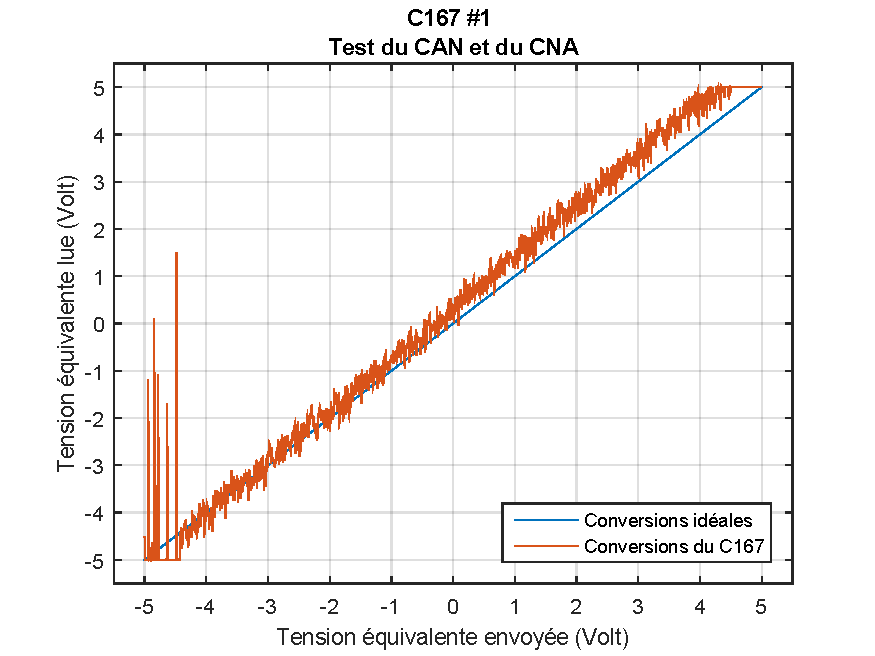
\includegraphics[width=.9\textwidth]{./V/images/CAN_CNA_mesures_1.pdf}
\caption{\label{fig:errCAN_1}Erreurs de conversions entre le CAN et le CNA (pour le C167 n°1)}
\end{minipage}\hfill%
\begin{minipage}[t]{.48\textwidth}
\centering 		
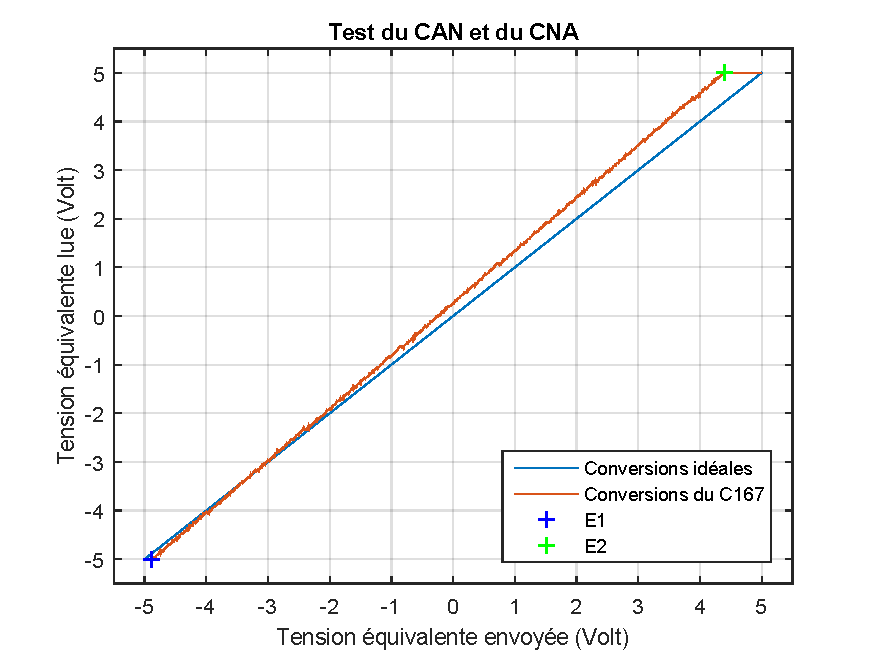
\includegraphics[width=.9\textwidth]{./V/images/CAN_CNA_mesures.pdf}
\caption{\label{fig:errCAN}Erreurs de conversions entre le CAN et le CNA (pour le C167 n°2)}
\end{minipage}
\end{figure}

Un protocole de test complet aurait été :\\
\begin{itemize}
\item Pour le CAN : 
	\begin{itemize}
		\item Générer, à partir d'un générateur de basse tension, un signal triangle de $0$ à $5$ Volt de fréquence faible.
		\item Lire toutes les valeurs et les faire afficher sur un terminal par le micro-contrôleur.
		\item Les comparer (à l'aide d'un tableur ou de Matlab) et vérifier la linéarité de la conversion.
		\item À partir des ces résultats, créer une fonction qui corrige les erreurs, si possible.
	\end{itemize}

\item Pour le CNA :
	\begin{itemize}
		\item Générer, à partir du micro-contrôleur un signal triangle de $-5$ à $5$ Volt de fréquence faible.
		\item Récupérer les valeurs à partir d'un CAN déjà corrigé (carte d'acquisition Matlab, ou le CAN précédemment si la correction donne de très bons résultats).
		\item Les comparer (à l'aide d'un tableur ou de Matlab) et vérifier la linéarité de la conversion.
		\item À partir des ces résultats, créer une fonction qui corrige les erreurs, si possible.
	\end{itemize}
\end{itemize}

%%%%%%%%%%%%%%%%%%%%%%%%%%%%%%%%%%%%%%%%%%%%% /!\  %%%%%%%%%%%%%%%%%%%%%%%%%%%%%%%%%%%
%%%%%%%%%%%%%%%%%%%%%%%%%%%%%%%%%%%%%%%%%%%%% /!\  %%%%%%%%%%%%%%%%%%%%%%%%%%%%%%%%%%%
%%%%%%%%%%%%%%%%%%%%%%%%%%%%%%%%%%%%%%%%%%%%% /!\  %%%%%%%%%%%%%%%%%%%%%%%%%%%%%%%%%%%\\
%%%%%%%%%%%%%%%%%%%%%%%%%%%%%%%%%%%%%%%%%%%%% /!\  %%%%%%%%%%%%%%%%%%%%%%%%%%%%%%%%%%%



\section{Transformation CAN/CNA}
\subsection{CAN}
Afin de réalisé notre commande, nous avons dût transformer la valeur entière lue pour $V_S$ par le CAN en un équivalent de la tension de type nombre à virgule flottante.  Figure \ref{fig:CAN_p}, nous pouvons observer les valeurs que peut convertir le CAN et les valeurs dont nous avons besoins. Nous n'utilisons ici que la moitié de la valeur lue par le convertisseur car nous n'avons besoin de convertir que des valeurs comprises entre $0$ et $5$ Volt. Ici, la plage de conversion est donc à moitié utilisée. 
Dans un premier temps, nous avons décaler la valeur lue (avec un et bit a bit) afin d'avoir la valeur sur $\left[ 0 , 1023\right]$,  puis  nous avons réalisé la conversion en tension avec l'équation \ref{equ:CAN1}.
\begin{figure}[!ht]%
\begin{minipage}{.5\textwidth}%
\centering
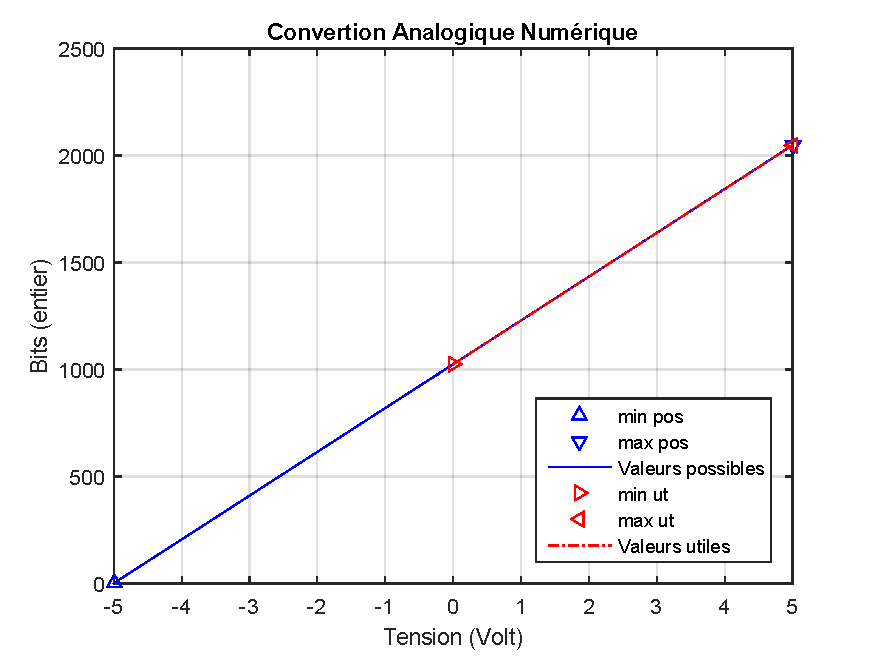
\includegraphics[width=\textwidth]{./VI/images/CAN_plage.pdf}
\caption{\label{fig:CAN_p}Valeurs possibles et possibles du CAN}
\end{minipage}%
\hfill%
\begin{minipage}{.5\textwidth}%
\begin{equation}
\begin{array}{l}
\left\lbrace
\begin{array}{lcl}
\label{equ:CAN1}V_{CANr} &=& V_{CAN} \&_{bàb} 1023\\
V_{volt} &=& \frac{5}{2^{10}-1}V_{CANr}
\end{array}
\right.\\
\Rightarrow V_{volt} = \frac{5}{2^{10}-1}( V_{CAN} \&_{bàb} 1023)
\end{array}
\end{equation}
\end{minipage}%
\end{figure}



\subsection{CNA}
La génération de la sortie $V_M$ nécessite aussi une conversion du CNA depuis la tension calculée par la commande (nombre à virgule flottante) vers un entier compris entre $-5$ et $5$ Volts. Néanmoins, la commande calcule une valeur comprise entre $-5$ et $5$ Volts, mais la carte de puissance branchée sur la sortie du CNA nécessite en entrée une tension comprise entre $0$ et $5$ Volt. Il faut donc, dans un premier temps, redresser la valeur calculée $V_{com}$ par la sortie sur une intervalle $\left[0;5\right]$ $V_{redr}$, puis le convertir en entier $V_{CNA}$. Pour cela nous utilisons les équations suivantes :

\begin{figure}[!ht]%
\begin{minipage}{.5\textwidth}%
\begin{equation}\label{eqn:CNA1}
\begin{array}{l}
\left\lbrace
\begin{array}{lcl}
V_{red}	&=&	\frac{1}{2}V_{com}+2,5\\
V_{CNA} &=& \frac{2^{11}-1}{5}V_{red}+2048\\
\end{array}
\right.\\
\Rightarrow V_{CNA} = \left\lfloor 204.7 V_{com} + 3071.5 \right\rfloor
\end{array}
\end{equation}	
\end{minipage}%
\hfill%
\begin{minipage}{.5\textwidth}%
\centering
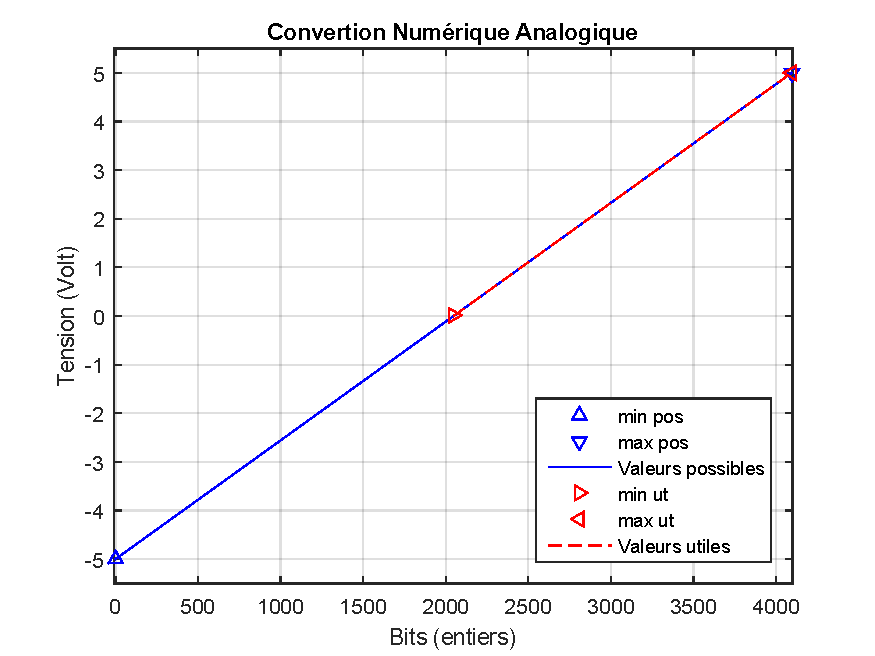
\includegraphics[width=\textwidth]{./VI/images/CNA_plage.pdf}
\caption{\label{fig:CNA_p}Valeurs possibles et possibles du CNA}
\end{minipage}%
\end{figure}

%	\subsection{Implémentation d'un programme de test des convertisseurs}
%	\subsection{Correction}
\section{Implémentation sur micro-contrôleur}	
Nous souhaitons dans cette partie vous présenter comment nous avons aborder l'implémentation des commandes sur le micro-contrôleur. Nous aborderons dans un premier temps une revue des tâches que nous avons utilisées. 
		\subsection{Description des taches}
		\paragraph*{Génération échelon}
		Une première tâche sera dédié à la génération d'un échelon. Nous souhaitons observer des changements de front de la consigne, c'est pourquoi il est intéressant de faire évoluer cette consigne périodiquement. Dans cette tâche, qui déroule du squelette obtenu sur les fichiers sources, nous allons avoir le déroulement suivant : \begin{itemize}
		\item[État 1] Valeur de la consigne mise à l'état haut. Variable d'état = 2
		\item[État 2] Valeur de la consigne mise à l'état bas. Variable d'état = 1
\end{itemize}
La fréquence d'appel de cette tâche n'a pas de grand impact sur les contraintes temps réel. Les timers ont déjà été programmé sur une fréquence de $f_{ech} = \frac{3.36}{2}Hz$, nous garderons ce résultat dans le reste de l'étude.		 
\paragraph{Acquisition des mesures}		 
		Cette tâche beaucoup plus principale que la précédente doit permettre de récupérer la valeur lue sur le CAN, calculer la commande associée et la transmettre au CNA. Ce déroulement a été décrit dans le schéma \ref{fig:GeneralSCHEMA}. Il est important de faire attention au conversion obtenu dans les équations \ref{eqn:CNA1} et \ref{equ:CAN1}.
		%	Acquisition 
		%	ref : CAN/CNA
		%         Conversion
		\subsection{Implémentation}
		Vous trouverez le code implémenté en langage C des tâches dans l'annexe \ref{Annex:codeC}. Nous avons aussi inclus un fichier de génération de paramètres via un modèle discret de $MATLAB$. Ce fichier génère un \emph{.txt} en fonction des paramètres de l'équation récurrente du prototype de commande.
		\subsection{Validation et correction}
		Nous avons obtenu des problèmes pour le prototype qui a été discrétisé dans la partie \ref{chap:Command} et qui est contenu dans le programme. Il semble que certaines problématiques nous ait échappé, notamment les notions de correction des CAN CNA évoquée dans \ref{sub:CAN_CNA}. Pour évaluer si le problème venait de la conversion, nous avons tout de même été capable de générer un échelon de tension qui vous est présenté dans la figure ci dessous. 
		\begin{figure}[!ht]
		\centering
		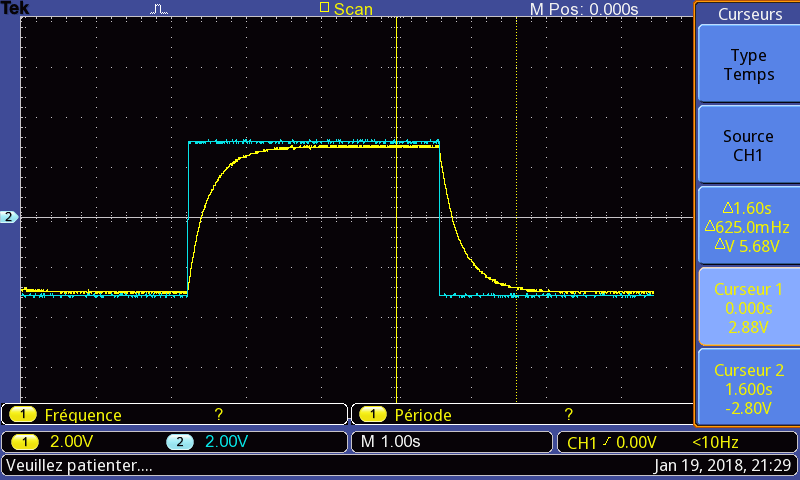
\includegraphics[width = .7\textwidth]{./VI/images/MicroC-reponseEchelon.png}
		\caption{Réponse à un échelon +2V, -2V}
\end{figure}				
		